 \documentclass[11pt,bibliography=totocnumbered]{article}
\usepackage[a4paper, hmargin={2.8cm, 2.8cm}, vmargin={2.5cm, 2.5cm}]{geometry}
\usepackage{eso-pic} % \AddToShipoutPicture
\usepackage{graphicx} % \includegraphics
\usepackage{framed}
\usepackage[utf8]{inputenc}
\usepackage{hyperref}
\usepackage{amsmath} % flere matematikkommandoer
\usepackage{amssymb} % flere matematikkommandoer
\usepackage{amsfonts}              % for blackboard bold, etc
\usepackage{amsthm}                % better theorem environments
\usepackage[utf8]{inputenc} % æøå
\usepackage[T1]{fontenc} % mere æøå
\usepackage{verbatim} % så man kan skrive ren tekst
\usepackage[all]{xy} % den sidste (avancerede) formel i dokumentet
\usepackage{graphicx}              % to include figures
\usepackage{caption}
\usepackage{bm}
\usepackage{fancyhdr}
\usepackage{mathtools}
\usepackage{listings}
\usepackage[inline]{enumitem}
\usepackage{color}
\usepackage[nottoc,numbib]{tocbibind}
\usepackage{tikz}
\usepackage{mdframed}
\usetikzlibrary{arrows,automata,fit,positioning, shapes, arrows.meta,chains,matrix,decorations.pathreplacing, calc}
\newcommand\doubleplus{+\kern-1.3ex+\kern0.8ex}
\newcommand\lett{\phantom{-}\:\:\mathbf{let}\:\:}
\newcommand\inn{\:\:\mathbf{in}\:\:}
%% Change `ku-farve` to `nat-farve` to use SCIENCE's old colors or
%% `natbio-farve` to use SCIENCE's new colors and logo.
\def \ColourPDF {include/nat-farve}

%% Change `ku-en` to `nat-en` to use the `Faculty of Science` header
\def \TitlePDF   {include/nat-en}  % University of Copenhagen

\title{
  \vspace{3cm}
  \Huge{Implementing Map-Scan Fusion in the Futhark Compiler} \\
  \Large{Bachelor project}
}

\author{
  \Large{Brian Spiegelhauer}
  \\ \texttt{brianspieg@gmail.com} \\ \\
   \Large{William Jack Lysgaard Sprent}
  \\ \texttt{bsprent@gmail.com} \\
}

\date{
    \today
}

\begin{document}
\lstset{language=C, frame=single, numbers=left, breaklines=true}
\mdfdefinestyle{alignbox}{leftmargin=100pt,
rightmargin=100pt,%
innerleftmargin=10pt,
innerrightmargin=10pt,
innertopmargin=0.1pt,
innerbottommargin=0.1cm,
skipbelow=10pt}

\AddToShipoutPicture*{\put(0,0){\includegraphics*[viewport=0 0 700 600]{\ColourPDF}}}
\AddToShipoutPicture*{\put(0,602){\includegraphics*[viewport=0 600 700 1600]{\ColourPDF}}}

\AddToShipoutPicture*{\put(0,0){\includegraphics*{\TitlePDF}}}

\clearpage\maketitle
\thispagestyle{empty}

\newpage

\tableofcontents

\newpage

\section{Abstract}
The ability to fuse loops together in a sequential program makes it possible to reduce loop overhead, increase execution speed and potentially optimise both memory hierarchy, time overhead, and space requirements. The effects of these optimisations -- especially memory related -- can have extended benefits when executing on a GPU. Futhark, a heavily optimising functional
 programming language aimed at GPU execution,
 exploits functional invariants to more easily perform loop fusion. We have expanded Futhark's fusion module to support:

\begin{itemize}
\item A new language construct, \texttt{scanomap}.
\item Producer-consumer fusion with \texttt{map} as producer and \texttt{scan} as consumer by using the \texttt{scanomap} construct.
\item Both producer-consumer fusion of \texttt{map} and \texttt{scanomap} expressions, and horizontal fusion of two \texttt{scanomaps}.
\end{itemize}
We show that by successfully fusing \texttt{map} and \texttt{scan} expressions, we enable significant speedup as a result of memory access optimisation. 
We demonstrate the effectiveness of our implementation on three different benchmark programs, displaying GPU execution time speedup in ranges of 1.2-1.5 times faster with our implementation.


These results suggest a significant potential in increase of performance from implementing fusion. Unleashing even more potential in GPGPU as well as improving big data calculations on CPU.
\section{Introduction}

The Futhark language is a functional programming with which the main idea is to allow for the expression of sufficiently complex programs while exploiting functional invariants such that
 programs can be aggressively optimised and have their parallelism exploited \cite{futharkdoc}. Its main target is to support general purpose computing on GPUs (GPGPU) to exploit their high parallel
 computational power.

Loop fusion is a method of identifying two or more loops in an iterative program which can be combined for potential speedup as a result of altering memory access patterns  or reducing loop overhead.
 The optimisation pipeline of the Futhark compiler already contains a fusion module; it futhermore supports a range of fusion optimisations by exploiting invariants in its Second Order Array Combinator (SOAC) constructs -- which are semantically identical
 to higher order functions found in functional languages \cite{T2Fusion}. The fusion module is not complete, but supports a range of SOAC fusions for example fusing two \texttt{map} expressions together. However, it does not currently support fusion between \texttt{map} and \texttt{scan} expressions.

For our project we will explore the possibility of implementing \texttt{map}-\texttt{scan} fusion into the Futhark compiler and will examine the performance benefits (if any) of performing such optimisations.

\subsection{Motivation}
Performing global memory accesses when performing computations on a GPU, due to their weaker caching system, is often far more penalising than on a CPU. Hence, performing loop fusion on a program
 which is to be on a graphics card, has the ``[...] potential to optimise both the memory hierarchy time overhead and, sometimes asymptotically, the space requirement'' \cite[p. 1]{T2Fusion} for the program as a result of 
improving memory access patterns and making temporary arrays obsolete \cite{T2Fusion}.
 Thus, the main motivation for adding \texttt{map}-\texttt{scan} fusion capabilities to
 the optimiser of the Futhark compiler is the potential for enabling speedups for relevant Futhark programs.

\subsection{Tasks}
The project can be divided into five main tasks:
\begin{enumerate}
    \item Gain an understanding of logical reasoning behind fusion optimisations on Second Order Array Combinators.
    \item Read and understand the relevant parts of the Futhark compiler required to make the necessary changes in the compiler.
    \item Modify all modules of the Futhark compiler necessary to implement the Map-Scan fusion itself.
    \item Benchmark the modified compiler against the unmodified compiler.
    \item Evaluate the results.
\end{enumerate}
Initially, these tasks look fairly straight forward. However, we expect that the main difficulties of this project lie within unforeseen roadblocks which we may encounter when modifying the codebase.

\section{Background Information}
%Describe some relevant background info for how SOACs are parallelly computed - relevant %to why Scanomap is smart. IMPORTANT: WHY MEMORY MANAGEMENT IS VERY IMPORTANT ON GPU\\
In the past decade or so the constant demand for more powerful CPUs has increasingly been satisfied through increasing the amount of cores rather than simply attempting to increase clock-speed.
 This trend of multi-core processors seeks to take advantage of latent potential for performing computational tasks in parallel -- with the aspiration being doubled performance when doubling the
 number of cores. At the same time graphics cards with GPUS containing up to thousands of cores have become mainstream, and while they have been designed for graphics rendering, their sheer degree of 
parallelism brings a great potential for general purpose computation. 

Reasoning about, and writing programs which exploit parallelism on GPUs can be a challenge, and parallel libraries such as CUDA and OpenCL, while useful, are not necessarily productive to work with directly.
 Hence, it is important to have languages which natively support parallel GPU execution, so that the compiler can handle many of the repeated challenges of writing parallel programs for the GPU, and 
 expedite the process of exploiting the GPU for computational power. The goal with Futhark is to fill this role by supplying a parallel language wherein specific compute intensive task can be defined and executed,
 lightening the load for a larger program written in a more general purpose language \cite{futharklang}.

This section will elaborate and detail what Futhark seeks to accomplish and how it does so.
% There are problems/calculations that gets to a size where normal sequential programming involving consecutive execution of processes, will reach a computation time unsatisfying for the intended users. In some cases these calculations can be done much faster with parallel programming. Parallel programming is where many calculations are carried out simultaneously, with the idea of dividing a problem into smaller sub problems solved at the same time. Parallel and sequential programming are not mutually exclusive, in the sense that if you use parallel programming, you cant use sequential programming, in many cases they are used together. Parallel programming can be done on the CPU with its multiple cores, but when possible and advantages it is much better to harness the thousands of cores in the GPU - graphics processing units. The GPU is no longer only used to do graphical calculations, but also General-purpose computing, GPGPU (General-purpose computing on graphics processing units). \\

% To do GPGPU, Hyperfit a joint research center addressing the simultaneous challenges of high transparency, high computational performance and high productivity in finance, employing an integrated approach of financial mathematics, domain specific languages, parallel functional programming, and high-performance systems \cite{Hyperfit} created Futhark. 


\subsection{Futhark}

Futhark is a ``statically typed, data-parallel, and purely functional array language'' \cite{futharklang} which aims to perform
 general purpose computing on GPUs (GPGPU). While Futhark is able to express imperative concepts such as in-place updates and loops, its main focus centred around the usage of
 functional language paradigm to express parallel computations through bulk operations using SOACs, which are semantically identical to higher order functions such as \texttt{map} and \texttt{reduce} commonly found in functional programming.

The Futhark compiler features an aggressive optimisation strategy which relies on strong, functional invariants found in constructs such as SOACs.

%Chunking
\subsection{SOACs}
Both \texttt{map} and \texttt{scan} are defined as SOACs -- or Second Order Array Combinators. Hence, they have no free variables, take first-order functions as arguments, and output first-order
 functions whose domains are arrays of the domain of the input.
While Futhark SOACs are semantically identical to their namesake higher-order functions found in other functional languages, working with SOACs allows for some assumptions to be made
 which turn out to be useful in regards to both parallelisation and optimisation. In particular each SOAC can be considered as representing a specific shape of an imperative do-loop, which
 is used in Futhark to expedite the loop-fusion process \cite[chap. 7]{MasterTroels}.

The intermediate representation of a Futhark program in the Futhark compiler does not contain arrays of tuples. Hence, when a Futhark program is compiled any expression of type $[\alpha]$ where
 $\alpha =  (\alpha_1, \alpha_2, ..., \alpha_n)$ is converted into an expression of type $([\alpha_1], [\alpha_2],..., [\alpha_n])$. Thus, we have that Futhark SOACs internally have an arbitrary amount
 of input arrays and output arrays. However, such notation can be cumbersome, so for the sake of clarity and ease we will notate tuples of arrays as single variables and types until the implementation
 section where it becomes relevant.
 For example, $b = \mathtt{map} \: f \: a$ is short hand for $(b0, b1,..., bn) = \mathtt{map} \: f \: (a0, a1, ..., am)$ where $ai$ and $bj$ are each arrays, and each of the arrays
 in a tuple have the same amount of
 elements.
% Definition of SOACs
% Why are they useful wrt. parallelisation
% Soacs with tuples in Futhark
\subsubsection{Map}
The $\texttt{map} \: f \: a$ function has the very simple definition of taking a function $f \: : \: \alpha \to \beta$ and returning a function $\mathtt{map} \:f \: : \: [\alpha] \to [\beta]$  which
 applies $f$ to every element of an input array, $a$.  This gives us the type signature of \texttt{map},
$$\mathtt{map} \: f \: a \: :  \: (\alpha \to \beta) \to [\alpha] \to [\beta]\mathnormal{.}$$
And the semantic definition of \texttt{map},
$$\mathtt{map} \: f \: a \: =  \: [f(a_0), f(a_1), ..., f(a_{n-1})]\mathnormal{.}$$
Having no free variables, means that each result $f(a_i)$ \textit{only} depends on the corresponding element $a_i$. This makes \texttt{map}s excellent for parallelisation because when the
 degree of parallelism reaches the size of $a$, $\mathtt{map} \: f \: a$ can potentially be computed in a single parallel step, or $c$ steps for a chunk size of $c$.

 \begin{figure}[h!]
   \centering
   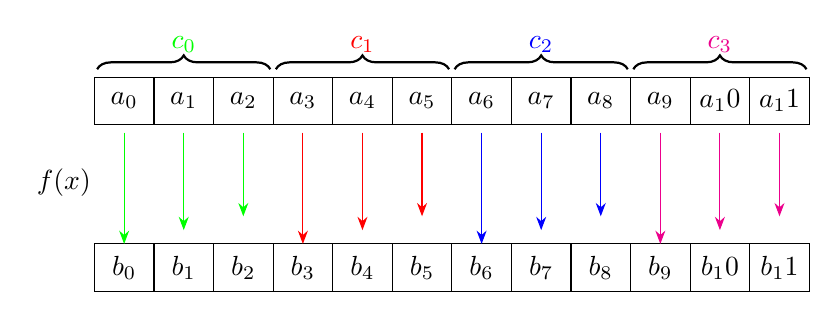
\begin{tikzpicture}[ node distance=0pt, start chain = A going
     right, start chain = C going right, arrow/.style =
     {draw=#1,-{Stealth[]}, shorten >=1mm, shorten
       <=1mm}, % styles of arrows
     arrow/.default = black, X/.style = {rectangle,
       draw,% styles of nodes in string (chain)
       minimum width=5ex, minimum height=4ex, outer sep=0pt, on
       chain}, B/.style = {decorate, decoration={brace, amplitude=5pt,
         pre=moveto,pre length=1pt,post=moveto,post length=1pt,
         raise=1mm, #1}, % for mirroring of brace, if necessary
       thick}, B/.default = mirror, % by default braces are mirrored
     ]
     \foreach \i in {0,...,11}% <-- content of nodes
     \node[X, on chain = A] {$a_\i$};

     \node [X, on chain = C, below = 10ex of A-1] {$b_0$}; \foreach \i
     in {1,...,11}% <-- content of nodes
     \node[X, on chain = C] {$b_\i$};

     ; \draw[B=] (A-1.north west) -- coordinate[above=3mm] (a1)
     (A-3.north east) node [green, midway, above, yshift = 5pt] (a)
     {$c_0$}; \draw[B=] (A-4.north west) -- coordinate[above=3mm] (a2)
     (A-6.north east) node [red, midway, above, yshift = 5pt] {$c_1$};
     \draw[B=] (A-7.north west) -- coordinate[above=3mm] (a3)
     (A-9.north east) node [blue, midway, above, yshift = 5pt]
     {$c_2$}; \draw[B=] (A-10.north west) -- coordinate[above=3mm]
     (a4) (A-12.north east) node [magenta, midway, above, yshift = 5pt]
     {$c_3$};


     \foreach \c [count=\i] in {green, red, blue, magenta} { \foreach
       \j in {1,...,3} { \pgfmathtruncatemacro{\is}{\i - 1}%
         \pgfmathtruncatemacro{\jn}{\is * 3 + \j}%
         \pgfmathtruncatemacro{\jl}{(\j - 1) * 5}%
         \draw[arrow,\c , shorten >= \jl pt] (A-\jn.south) to
         (C-\jn.north) node (AR-\jn) {}; } }

     \node [above left= 10pt and 5pt of AR-1] {$f(x)$};

   \end{tikzpicture}
   
   \caption{Parallel computation of map with chunking. Each colour represents a separate thread.}
   \label{fig:compmap1}
 \end{figure}

Figure \ref{fig:compmap1} displays how \texttt{map} can be computed in chunks. Each thread is responsible for sequentially computing
 $\mathtt{map} \: f \: c_i$ across a single chunk. With no dependencies in the way, this can happen in parallel such that the
 12 element list is \texttt{map}ped with just three sequential applications of $f$.
% INSERT COOL FIGURE OF MAP BEING COMPUTED 
% How do we compute it parallely
% Timecomplexity?

\subsubsection{Scan}
% what is a scan
$\texttt{scan} \: \odot \: e \: a$ takes a binary, associative function $\odot \: : \: \alpha \to \alpha \to \alpha$ and returns a function
 $\mathtt{scan} \:\odot \: : \: \alpha \to [\alpha] \to [\alpha]$ which
 computes the $\odot$ prefixes of an input array $a$ starting with a neutral element, $e$. Overall, \texttt{scan} has the type signature,
$$\mathtt{scan} \: \odot \: e \: a \: : \:(\alpha \to \alpha \to \alpha) \to \alpha \to [\alpha] \to [\alpha]\mathnormal{.}$$
Computing \texttt{scan} with the function $\odot$, the array $a$, and neutral element $e$ gives us,
$$\mathtt{scan} \: \odot \: e \: a \: = [e \odot a_0, e \odot a_0 \odot a_1, ..., e \odot a_0 \odot ... \odot a_{n-1}]\mathnormal{.}$$
% How do we compute it parallely
However, computing such a \texttt{scan} is not as simple as with a \texttt{map} as each prefix $a_0 \odot ... \odot a_i$ obviously depends on the previous prefix $a_0 \odot ... \odot a_{i-1}$. Accordingly, 
the associativity of $\odot$ is vital as it means that this dependency does not force computation order, and partial results can be computed independently and combined.
% How scan is computed in Futhark with fancy diagram 

% Timecomplexity?
\begin{figure}[h!]
  \centering
  \begin{tikzpicture}[ node distance=0pt,
    start chain = A going right,
    start chain = C going right,
    start chain = D going right, 
    start chain = E going right,
    start chain = G going right,
    arrow/.style = {draw=#1,-{Stealth[]},shorten >=1mm, shorten <=1mm}, % styles of arrows
    arrow/.default = black, X/.style = {rectangle, draw,% styles of nodes in string (chain)
      minimum width=7ex, minimum height=4ex, outer sep=0pt, on chain},
    B/.style = {decorate, decoration={brace, amplitude=5pt,
        pre=moveto,pre length=1pt,post=moveto,post length=1pt,
        raise=1mm, #1}, % for mirroring of brace, if necessary
      thick},
    B/.default = mirror, % by default braces are mirrored
    ]
    \foreach \i in {0,...,11}% <-- content of nodes
    \node[X, on chain = A] {$a_\i$};

    \node [X, on chain = C, below = 10ex of A-1] {$a_0$};
    \node [X, on chain = C] {$a_{0-1}$};
    \node [X, on chain = C] {$a_{0-2}$};
    \foreach \i in {3, 6, 9} { 
      \node[X, on chain = C] {$a_\i$};
      \foreach \j in {1,...,2} { 
        \pgfmathtruncatemacro{\ij}{\i + \j}%%
        \node[X, on chain = C] {$a_{\i-\ij}$}; 
      }
    }

    \node [X, on chain = D, below = 10ex of C-1] {$a_0$};
    \node [X, on chain = D] {$a_{0-1}$};
    \node [X, on chain = D] {$a_{0-2}$};
    \node [X, on chain = D] {$a_{3}$};
    \node [X, on chain = D] {$a_{3-4}$};
    \node [X, on chain = D] {$a_{0-5}$};
    \node [X, on chain = D] {$a_{6}$};
    \node [X, on chain = D] {$a_{6-7}$};
    \node [X, on chain = D] {$a_{3-8}$};
    \node [X, on chain = D] {$a_{9}$};
    \node [X, on chain = D] {$a_{9-10}$};
    \node [X, on chain = D] {$a_{6-11}$};

    \node [X, on chain = E, below = 10ex of D-1] {$a_0$};
    \node [X, on chain = E] {$a_{0-1}$};
    \node [X, on chain = E] {$a_{0-2}$};
    \node [X, on chain = E] {$a_{3}$};
    \node [X, on chain = E] {$a_{3-4}$};
    \node [X, on chain = E] {$a_{0-5}$};
    \node [X, on chain = E] {$a_{6}$};
    \node [X, on chain = E] {$a_{6-7}$};
    \node [X, on chain = E] {$a_{0-8}$};
    \node [X, on chain = E] {$a_{9}$};
    \node [X, on chain = E] {$a_{9-10}$};
    \node [X, on chain = E] {$a_{0-11}$};




    \node [X, on chain = G, below = 10ex of E-1] {$a_0$};
    \node [X, on chain = G] {$a_{0-1}$};
    \node [X, on chain = G] {$a_{0-2}$};

    \foreach \i in {3,...,11} {
      \node[X, on chain = G] {$a_{0-\i}$};
    }


    \draw[B=] (A-1.north west) -- coordinate[above=3mm] (a1)
    (A-3.north east) node [green, midway, above, yshift = 5pt] (a)
    {$c_0$}; \draw[B=] (A-4.north west) -- coordinate[above=3mm] (a2)
    (A-6.north east) node [red, midway, above, yshift = 5pt] {$c_1$};
    \draw[B=] (A-7.north west) -- coordinate[above=3mm] (a3)
    (A-9.north east) node [blue, midway, above, yshift = 5pt] {$c_2$};
    \draw[B=] (A-10.north west) -- coordinate[above=3mm] (a4)
    (A-12.north east) node [magenta, midway, above, yshift = 5pt]
    {$c_3$};


    \foreach \c [count=\i] in {green, red, blue, magenta} {
      \foreach \j in {2,...,3} { 
        \pgfmathtruncatemacro{\is}{\i - 1}%
        \pgfmathtruncatemacro{\jn}{\is * 3 + \j}%
        \pgfmathtruncatemacro{\jl}{(\j - 2) * 5}%
        \draw[arrow,\c , shorten >= \jl pt] (A-\jn.south) to (C-\jn.north) node (AR-\jn) {};
      }
    }
    \foreach \c [count=\i] in {green, red, blue, magenta} {
      \foreach \j in {1,...,2} {
        \pgfmathtruncatemacro{\ir}{\i - 1}%
        \pgfmathtruncatemacro{\pos}{3 * \ir + \j}%
        \pgfmathtruncatemacro{\ii}{\pos +1}%
        \draw[arrow, \c] (A-\pos.south) to[out=280, in=200] (A-\ii.south) node (CR-\pos) {};
      }
    }
    \foreach \i/\c in {3/red,6/blue,9/magenta} {
      \pgfmathtruncatemacro{\iii}{\i + 3}%
      \def\this{C-\iii.south}
      \def\there{D-\iii.north}
      \coordinate (mid\i) at ($(\this) !0.6! (\there)$);
      \node at (mid\i) {$\odot$};
      \draw[arrow, \c,shorten >= 4pt] (C-\iii.south) to node[midway, black] (RED-1) {} (mid\i.north) ;
      \draw[arrow, \c,shorten >= 4pt] (C-\i.south) to[out=340 ,in=90] (mid\i.north);
      \draw[arrow, \c,shorten <= 4pt] (mid\i) to (D-\iii.north) ;

    }


    \foreach \i/\c in {3/blue,6/magenta} {
      \pgfmathtruncatemacro{\iii}{\i + 6}%
      \def\this{D-\iii.south} 
      \def\there{E-\iii.north}
      \coordinate (mid\i) at ($(\this) !0.6! (\there)$);
      \node at (mid\i) {$\odot$};
      \draw[arrow, \c,shorten >= 4pt] (D-\iii.south) to node[midway, black] (RED-1) {} (mid\i.north) ;
      \draw[arrow, \c,shorten >= 4pt] (D-\i.south) to[out=320 ,in=90, looseness=0.6] (mid\i.north);
      \draw[arrow, \c,shorten <= 4pt] (mid\i) to (E-\iii.north) ; 
    }




    \foreach \c [count=\i] in {red, blue, magenta} {
      \foreach \j in {2,...,3} {
        \pgfmathtruncatemacro{\is}{\i - 0}%
        \pgfmathtruncatemacro{\jn}{\is * 3 + \j -1}%
        \pgfmathtruncatemacro{\jl}{(\j - 2) * 3}%
        \draw[arrow,\c, shorten >= \jl pt] (E-\jn.south) to (G-\jn.north) node (GR-\jn) {};
      }
      \foreach \j in {1,...,2} { 
        \pgfmathtruncatemacro{\ir}{\i - 1}%
        \pgfmathtruncatemacro{\star}{3 * \ir + 3}%
        \pgfmathtruncatemacro{\pos}{3 * \ir + \j + 2}%
        \pgfmathtruncatemacro{\ii}{\pos +1}%
        \draw[arrow, \c] (E-\star.south) to[out=280, in=200] (E-\ii.south) node (GGR-\pos) {};
      }
    }
    \node [above left= 10pt and 5pt of AR-1] (other) {$\odot$};
    \node [below= 38ex of other] {$\odot$};
  \end{tikzpicture}
  
  \caption{Parallel computation of \texttt{scan} with chunking. Each colour represents a single thread, and $a_{i-j} = a_i \odot a_{i+1} \odot ... \odot a_j$.}
  \label{fig:scancomp1}
\end{figure}
Thus, there are multiple ways in which \texttt{scan} can be computed in parallel with chunking, and Figure \ref{fig:scancomp1} shows a simple algorithm.
 It is a three phase process which step-wise involves,
 \begin{enumerate}
 \item Each thread sequentially computes the $\odot$-prefixes of their respective chunks. ($c$ steps)
 \item Then the final element of each chunk is recursively combined with the previous using $\odot$ with
 doubling stride for each recursion, such that each final element contains the $a_{0-j}$ prefix where $j = (c * (i+1) - 1)$ for the
 $i$th chunk. ($\log(\frac{n}{c})$ steps)
 \item Each thread adds the final element of the previous chunk to each element of the chunk
 which is not the tail. ($c$ steps)
 \end{enumerate}
While this algorithm is not work efficient -- it involves more than $n$ applications of $\odot$ -- it still has a depth of $O(2c + \log(\frac{n}{c})) < O(n)$ due to parallelism.
 This also shows the idea of chunking, for example in Figure \ref{fig:scancomp1}, if we instead of having four threads to compute the scan, had $12$ -- or $n$ threads in general -- we
 could exploit this by simply setting the chunk-size to $c = 1$. This would forego steps 1 and 3, giving us a total depth of $O(\log(n))$.

\subsubsection{Loop Conversion}
Each SOAC can always be converted to an equivalent loop. For example, both $b = \mathtt{map} \: f \: a$ and
and $b = \mathtt{scan} \: g \: e \: a$ can be converted into equivalent loops (see Listing \ref{lst:maploop} \& \ref{lst:scanloop}).
\begin{lstlisting}[caption=\texttt{map} as a loop., label={lst:maploop}]
  b[n];
  for (i = 0; i < n; i++) {
    b[i] = f(a[i])
  }
\end{lstlisting}
\begin{lstlisting}[caption=\texttt{scan} as a loop., label={lst:scanloop}]
  b[n];
  acc = e;
  for (i = 0; i < n; i++) {
    acc = g(acc, a[i])
    b[i] = acc
  }
\end{lstlisting}

However, such a conversion comes with a loss of useful invariants. For example, we can always rely on a loop created from a \texttt{map} expression to have no cross-iteration
 dependencies; each iteration will not depend on a result computed in another iteration. This means that a \texttt{map}-loop can always be computed in parallel. On the other hand,
 deciding whether or not a generic loop can be computed in parallel requires sometimes complex dependency analysis.

\section{Fusion}
In this section, the basic idea of loop fusion will be outlined, with a closer look at the two kinds of fusion implemented in this paper.
The loop fusion technique gives the possibility of
\begin{enumerate*}[label=\alph*)]
\item reducing loop overhead,
\item increasing execution speed, and
\item the potential to optimise both the memory hierarchy time overhead and space requirements.
\end{enumerate*}
 As the name implies, loop fusion consists of fusing loops together. However this requires that the loops iterate the same number of times, as that could for example make one loop try to fetch data out of bounds.

Having two loops with the same iteration range as shown in Listing \ref{lst:horipre}, it gives the possibility for fusion them together as one. Both loops do the work needed within the same range, and therefore it could be done in one loop as shown in Listing \ref{lst:horipost}. Cases where fusion will not be possible regardless of two equal length loops, will be shown later on.

By doing the fusion in this case, loop-overhead has been reduced in half, as it's now only necessary to keep track of one loop instruction.

\subsection{Consumer-Producer Fusion}
Producer-consumer loop fusion is slightly more complicated. In this case the two loops are connected, as in inside the producer-loop some data is being created, that is required in the consumer-loop; a producer creates some data, and a consumer uses the created data.
 Ergo the relationship is referred to as a producer-consumer relationship.

Loop fusion of a producer-consumer relationship thus gives the opportunity to fuse the functions in the two loops into one, i.e $f(x) \circ g(x) = f(g(x))$ as the example in listing \ref{lst:pc-pre} and \ref{lst:pc-post}.

The result is reduced loop overhead, reducing in memory requirements as the output of the producer loop is no longer stored separately, but calculated within the fused result.

\begin{lstlisting}[caption=Producer-Consumer pre-fusion.,label={lst:pc-pre}] 
  a[n];
  b[n];
  c[n];
  	  
  for (int i = 0; i < n; i++) {
    b[i] = f(a[i])
  }
  
  for (int i = 0; i < n; i++) {
    c[i] = g(b[i])
  }
\end{lstlisting}

\begin{lstlisting}[caption=Producer-Consumer post-fusion.,label={lst:pc-post}] 
  a[n];
  c[n];
  	  
  for (int i = 0; i < n; i++) {
    c[i] = f(g(a[i])
  }
\end{lstlisting}

\subsection{Horizontal Fusion}
Horizontal fusion is a none producer-consumer fusion, i.e the two loops must have no connection with each other; Listing \ref{lst:horipre} and \ref{lst:horipost} therefore perfectly examplify a horizontal fusion.  
\begin{lstlisting}[caption=Pre-fusion,label={lst:horipre}]

  a[n];
  b[n];

  for (int i = 0; i < n; i++) {
    a[i] = i
  }

  for (int i = 0; i < n; i++) {
    b[i] = i
  }
\end{lstlisting}

\begin{lstlisting}[caption=Post-fusion,label={lst:horipost}]
  a[n];
  b[n];
  
  for (int i = 0; i < n; i++) {
    a[i] = i
    b[i] = i  
  }
\end{lstlisting}

\subsection{Fusion Hindrances}
Fusing a producer loop into a consumer loop is not always valid, and deciding whether or not a producer-consumer loop pair is safely fusible requires loop dependency analysis for every statement 
 in the consuming loop, such that dependencies can be upheld in a fused loop.
 For example, in Listing \ref{lst:dep1pre} we can see that statement \texttt{S2} depends on iteration $i$ of \texttt{S1} and iteration $i-1$ of \texttt{S2}. Thus loop \texttt{a} can safely be fused together
 with loop \texttt{b}.

\begin{lstlisting}[caption=Example dependencies,label={lst:dep1pre}]
  a[n];
loop a:
  for (int i = 0; i < n; i++) {
S1: a[i] = f(i)
  }
  b[n];
loop b:
  for (int i = 0; i < n; i++) {
S2: b[i] = b[i - 1] + a[i]  
  }
\end{lstlisting}
However, in Listing \ref{lst:dep2pre} we have that statement \texttt{S4} depends on iteration $i+1$ of statement \texttt{S3}. If we were to fuse loop \texttt{c} and loop \texttt{d} into a single loop, then we would
 have a situation where \texttt{S4} would depend on a future iteration of its own loop. Hence, the result of fusing loops \texttt{c} and \texttt{d} would be an invalid program, and as such it is unsafe to fuse them.
\begin{lstlisting}[caption=Example dependencies,label={lst:dep2pre}]
  a[n];
loop c:
  for (int i = 0; i < n; i++) {
S3: c[i] = f(i)
  }
  b[n];
loop d:
  for (int i = 0; i < n; i++) {
S4: d[i] = c[i + 1]  
  }
\end{lstlisting}
With larger and more complicated loops, this kind of analysis can become very sophisticated and complicated. This is why we reason about fusion through SOACs as their shapes and dependencies as loops
 are well-known.
\subsection{Fusion in Futhark}
Futhark is centred around SOACs for doing operations on arrays, and generally loops aren't used to perform array computation. Loop fusion for that reason is focused on SOAC fusion. The SOACs can currently be divided as producer consumer functions as shown in Table 1.
\clearpage

\begin{table}[hb!]
\centering
\caption{Producers and Consumers in Futhark}
\label{my-label}
\begin{tabular}{|l|l|}
\hline
\textbf{Producers} & \textbf{Consumers} \\ \hline
Map                & Map                \\ \hline
                   & Reduce             \\ \hline
                   & Scan               \\ \hline
Filter             & Filter             \\ \hline
                   & Redomap            \\ \hline
                   & Scanomap           \\ \hline
\end{tabular}
\end{table}

This brings us to the benefits of reasoning about fusion via SOACs. Instead of being a question of ``can loop a be fused with loop b?'' we instead ask whether one type of SOAC can
 be fused with another. For example, take \texttt{map}-\texttt{map} producer-consumer fusion; we know that the program,
 \begin{align*}
   \lett b &= \mathtt{map} \: f \: a \inn \\
   \lett c &= \mathtt{map} \: g \: b \inn
 \end{align*}
can be expressed as the loops in Listing \ref{lst:mapmappre}
 and through dependency analysis we find that we can fuse those loops into the loop from Listing \ref{lst:mapmappost}.
\begin{lstlisting}[caption=\texttt{map} and \texttt{map} as producer and consumer, label={lst:mapmappre}]
  a[n];  	  
  b[n];
  for (int i = 0; i < n; i++) {
    b[i] = f(a[i]);
  }
  c[n];
  for (int i = 0; i < n; i++) {
    c[i] = g(b[i]);
  }
\end{lstlisting}
\begin{lstlisting}[caption=Loop from Listing \ref{lst:mapmappre} fused as producer and consumer, label={lst:mapmappost}]
  a[n];  	  
  c[n];
  for (int i = 0; i < n; i++) {
    c[i] = g(f(a[i]));
  }
\end{lstlisting}
The process above is equivalent to looking at the original SOAC statements, removing the intermediate array, and performing function composition on $f$ and $g$. If
 we do this, we get the following -- which if converted to a loop gives the exact same loop as Listing \ref{lst:mapmappost}.
 \begin{align*}
   \lett c &= \mathtt{map} \: (g \circ f) \: a \inn
 \end{align*}
\section{Map-Scan Fusion}
% Why?
In a typical situation involving \texttt{map} and \texttt{scan}, we will have the \texttt{map} producing some array, which is subsequently
 consumed by the \texttt{scan}:
\begin{align*}
  b &= \mathtt{map} \: f \: a \\
  c &= \mathtt{scan} \: \odot \: e \: b\mathnormal{.}
\end{align*}
To demonstrate the benefits of fusing these expressions, we can describe them in sequential code as two loops where the first produces the $b$ array and the second consumes $b$ to create $c$.
\begin{lstlisting}[caption=\texttt{map} and \texttt{scan} as sequential loops.]
  a[n];
  ...
  b[n];
  for (int i = 0; i < n; i++) {
    b[i] = f(a[i]);
  }
  c[n];
  acc = e;
  for (int i = 0; i < n; i++) {
    acc = g(acc, b[i]);
    c[i] = acc;
  }
\end{lstlisting}
In this situation, the memory access pattern will look something like the following,
\begin{align*}
  \mathtt{load}[a_0]&, \mathtt{store}[b_0], \mathtt{load}[a_1], \mathtt{store}[b_1], ..., \mathtt{load}[a_{n-1}], \mathtt{store}[b_{n-1}] \\
  \mathtt{load}[b_0]&, \mathtt{store}[c_0], \mathtt{load}[b_1], \mathtt{store}[c_1], ..., \mathtt{load}[b_{n-1}], \mathtt{store}[c_{n-1}]\mathnormal{.}
\end{align*}
However, if the $b$ array is not used outside the second loop, we can recall that the elements of the scanned array $c$ depend only on the previous prefixes. 
Hence, we have that $c_i$ will only depend on $b_j$ for $j \leq i$ being calculated. This gives us the option of fusing the two loops into a single loop which directly calculates $c$ from $a$.
\begin{lstlisting}[caption=\texttt{map} and \texttt{scan} loops fused.]
  a[n];
  ...
  b;
  c[n];
  acc = e;
  for (int i = 0; i < n; i++) {
    b = f(a[i]);
    acc = g(acc, b);
    c[i] = acc;
  }
\end{lstlisting}
Now, we have removed all accesses to $b$, giving us an access pattern as follows,
 $$\mathtt{load}[a_0],  \mathtt{store}[c_0], ..., \mathtt{load}[a_{n-1}],  \mathtt{store}[c_{n-1}]\mathnormal{.}$$
This is the goal of performing \texttt{map}-\texttt{scan} fusion. By fusing a \texttt{map} into a \texttt{scan}, we can optimise a program by eliminating costly memory accesses,
 which is even more useful when working on a GPU, which generally does not have the more forgiving memory hierarchy and caching system of a CPU.
\subsection{Scanomap}
% Naive approach
When looking to fuse a \texttt{map} into a \texttt{scan}, the most straightforward approach is to perform function
 composition on the input functions of the respective functions, turning the following,
\begin{align}
  b &= \mathtt{map} \: f \: a \\
  c &= \mathtt{scan} \: \odot \: e \: b
\intertext{into,}
  c &= \mathtt{scan} \: \odot_f \: e \: a
\end{align}
where, $$\odot_f \stackrel{\text{def}}{=} \odot \circ f$$
hence,
$$\odot \circ f = x \odot f(y)$$
 would be the naive approach.
However, the type signature of the resulting function $$\odot_f \: : \: \alpha \to \beta \to \alpha$$
 is not compatible with the Futhark definition of \texttt{scan}, and neither is it associative. Clearly, a different approach
 is needed.

The solution to this problem is to exploit how Futhark uses chunking. Since the associativity of the \texttt{scan} operator only
 comes into play during the parallel phase of computation, we can distinguish between how each chunk is computed sequentially and
 how chunks are joined.

To do so, we must expand the list of SOACs with the internal \texttt{scanomap} function. \texttt{Scanomap} is semantically similar
 to \texttt{scan}, however, it takes two function parameters;
 \begin{enumerate*}[label=\alph*)]
 \item an associative scanning function meant for parallelly scanning
   across chunks, and
 \item a sequential folding function meant for scanning
   within a chunk.
 \end{enumerate*}
\texttt{Scanomap} has the following type signature,
$$\mathtt{scanomap} \: \odot \: \odot_f \: e \: a \: : \:(\alpha \to \alpha \to \alpha) \to (\alpha \to \beta \to \alpha)
 \to \alpha \to [\beta] \to [\alpha]\mathnormal{.}$$
and can be considered semantically similar to performing a left fold with the $\odot_f$ function
$$\mathtt{scanomap} \: \odot \: \odot_f \: e \: a \: =
 [e \odot_f a_0, (e \odot_f a_0) \odot_f a_1, ..., ((e \odot_f a_0) \odot_f ...) \odot_f a_{n-1}]$$
which also corresponds to the chunk-wise computation of \texttt{scanomap}. The scanning operator can then be used to
 join two chunks,
$$\mathtt{scanomap} \: \odot \: \odot_f \: e \: (a \doubleplus b) \: = 
[a_0', a_1', ..., a_{n-1}'] \doubleplus [b_0' \odot a_{n-1}',b_1' \odot a_{n-1}', ...,b_{n-1}' \odot a_{n-1}']$$
where 
\begin{align*}
  \mathtt{scanomap} \: \odot \: \odot_f \: e \: a \: &= 
[a_0', a_1', ..., a_{n-1}']
\intertext{and}
  \mathtt{scanomap} \: \odot \: \odot_f \: e \: b \: &= 
[b_0', b_1', ..., b_{n-1}']\mathnormal{.}
\end{align*}

For \texttt{scanomap} to be used in facilitating \texttt{map}-\texttt{scan} fusion, we first observe that we have the
 following equivalence,
$$\mathtt{scan} \: \odot \: e \: a \equiv \mathtt{scanomap} \: \odot \: \odot \: e \: a \mathnormal{.}$$
Ergo, we can freely turn any regular \texttt{scan} into an equivalent \texttt{scanomap}. If we look to our previous example,
 we can see how a \texttt{map} can be fused into a \texttt{scan} using the \texttt{scanomap} construction:
\begin{align*}
  b &= \mathtt{map} \: f \: a \\
  c &= \mathtt{scan} \: \odot \: e \: b
\intertext{Firstly, we turn the \texttt{scan} into an equivalent \texttt{scanomap},}
  c &= \mathtt{scanomap} \: \odot \: \odot \: e \: b
\intertext{and then, secondly, compose a folding function, $\odot \circ f = \odot_f$, from the mapping function and the scanning operator and discard
 the intermediate $b$ list to arrive at an equivalent \texttt{scanomap},}
  c &= \mathtt{scanomap} \: \odot \: \odot_f \: e \: a\mathnormal{.}
\end{align*}
Any producer \texttt{map} can be fused into a consuming \texttt{scan} in this manner.
% Why do we need the scanomap construction?
% What is the Scanomap construction. What are its semantics, and why is it used.
% Show equivalence between a Scanomap and a composition of a map and a scan - similar to showing redomap results from a reduce . map.

\subsection{Necessary Conditions}
% Copy from T2/Troels.
Fusion is not always viable as there are some situations where fusion cannot or should not happen. Figure \ref{fig:cases} shows six cases where fusion transformation should not happen.

\begin{figure}[hb]
  \centering
    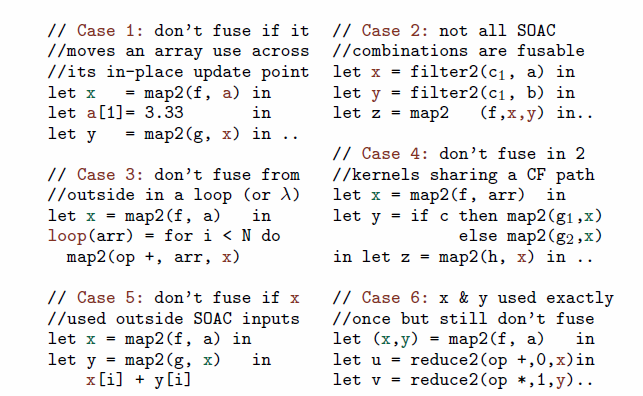
\includegraphics[width=0.6\textwidth]{images/cases.png}
  \caption{Don't Fuse Cases \cite[p. 6]{T2Fusion}}
  \label{fig:cases}
\end{figure}

\begin{itemize}
\item[Case 1:] Fusion across an in-place update is not possible -- i.e. $a[i] = k$. When fusing the producer array is not created as before, but a part of the computation in the resulting fused SOAC.
\item[Case 2:] Not all combinations of SOACs are fusible.
\item[Case 3:] Fusion across a loop or a SOAC lambda would duplicate the computation and potentially change the time complexity of the program. In this case instead of calculating variable $x$ once, a fusion would result in $x$ being calculated in each of the loops. 
\item[Case 4:] When the array $x$ produced by a SOAC is consumed by two other SOACs located on the same execution path, the computation will be duplicated.
\item[Case 5:] If array $x$ produced by SOAC is used other than input to another SOAC fusion is not allowed.
\item[Case 6:] If two arrays created by a SOAC, are used as input in more than one SOAC, the computation is duplicated, and fusion is therefore not allowed.\\ \cite[p. 6]{T2Fusion}
\end{itemize}

However there are special cases for scanomap, as the result array $x$ of the producer SOAC in the scanomap transformation, will also be returned by the scanomap in cases where other SOACs consumes array $x$.


\subsection{Fusing Scanomap}
% What can we not reduce with
Once a \texttt{map} and a \texttt{scan} have been combined into a \texttt{scanomap}, it raises the question of how one can further fuse this new construct.
 This section details which SOACs \texttt{scanomap} can fuse with and how.
\paragraph{Map-Scanomap Fusion:}
Fusing a \texttt{map} as a producer into a consumer \texttt{scanomap} is a simple process. Given a \texttt{map} with function $g$ and a 
 \texttt{scanomap} with the folding function $\odot_f$, we compose a new folding function $x \odot_{f \circ g} y = x \odot f (g (y))$. This is illustrated below,
\begin{align*}
  b &= \mathtt{map} \: g \: a \\
  c &= \mathtt{scanomap} \: \odot \: \odot_f \: e \: b \\
\Downarrow \\
  c &= \mathtt{scanomap} \: \odot \: \odot_{f\circ g} \: e \: a\mathnormal{.}
\end{align*}

\paragraph{Scanomap-Scanomap Fusion:} Horizontally fusing a \texttt{scanomap} with another \texttt{scanomap}, requires no dependency exists between the
 two SOACs -- i.e. there exists no producer-consumer relationship between the two. In theses cases, it may still prove beneficial to perform fusion -- even though there is no direct
 optimisation -- to enable more fusion.
% Tuples
This kind of fusion is performed by concatenating input, output, and both functions for the input \texttt{scanomaps}, which gives the following,
\begin{align*}
  c &= \mathtt{scanomap} \: \odot_1 \: {\odot_1}_f \: e_1 \: a \\
  d &= \mathtt{scanomap} \: \odot_2 \: {\odot_2}_g \: e_2 \: b \\
\Downarrow \\
  (c,d) &= \mathtt{scanomap} \: \odot' \: \odot'_{fg} \: (e_1, e_2) \: (a, b)\mathnormal{.}
\end{align*}
Where $\odot'(e_1,e_2, x, y) = (e_1 \odot x, e_2 \odot y)$ and $\odot'_{fg}(e_1, e_2, x, y) = (e_1 \odot f(x), e_2 \odot f(y))$. In this way, the resulting \texttt{scanomap}
 now describes the computations of both input \texttt{scanomap}s.
\section{Implementation}\label{sec:imp}
% How does a futhark program look ~ absyn. As we need it.
This section will detail the specifics of performing \texttt{map-scan}, and other \texttt{scanomap} fusions, as well as detailing the process of
analysing a program for valid fusions.

\subsection{Program State}
We make some assumptions regarding the internal representation of the program once it reaches the fusion module. The fusion module assumes a normalised program, with the following properties: 
\begin{quote}
\begin{itemize}
\item No tuple type can appear in an array or tuple type, i.e., flat
tuples,
\item tuple expressions can appear only as the final result of a function,
SOAC, or if expression, and similarly for the tuple pattern
of a let binding, e.g., a formal argument cannot be a tuple,
\item $\: e_1$ cannot be a let expression when used in let $\: p$ = $\: e_1$ in $\: e_2$,
\item each if is bound to a corresponding let expression, and
an if’s condition cannot be in itself an if expression, e.g., \\
$\: a$ + if( if $\: c_1$ then $\: e_1$ else $\: e_2$ ) then $\: e_3$ else $\: e_4$ $\rightarrow$ \\
let $\: c_2$ = if $\: c_1$ then $\: e_1$ else $\: e_2$ in \\
let $\: b$ = if $\: c_2$ then $\: e_3$ else $\: e_4$ in $\: a+ \:b$ 
\item function calls, including SOACs, have their own let binding, e.g., \\
reduce2($\:f,\:a$) + $\:x$ $\Rightarrow$ let $\:y$ = reduce2($\:f,\:e,\:a$) in $\:y+\:x$,
\item all actual arguments are vars, e.g., $\:f(\:a+\:b))$ $\Rightarrow$ let $\:x=\:a+\:b$ in $\:f(\:x)$.\\ \cite[Figure 5, p.4]{T2Fusion}
\end{itemize}
\end{quote} 
The properties listed above are reached by going through the different stages in the compiler pipeline, as shown in Figure \ref{fig:pipeline}.
\begin{figure}[hb!]
  \centering
    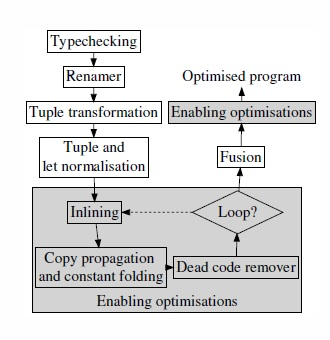
\includegraphics[width=0.5\textwidth]{images/pipeline.jpg}
  \caption{Compiler pipeline \cite[p. 4]{T2Fusion}}
  \label{fig:pipeline}
\end{figure}

\subsection{Bottom Up Analysis}
% How the fusion module analyses the program
The fusion module of the Futhark compiler gathers fusible SOACs by using a bottom-up analysis pass of the program's Abstract Syntax Tree (AST). This is done by traversing the AST depth-first, while using a set
 of environments and data structures, to among other things keep track of created kernels and the production and consumption of arrays \cite{T2Fusion}.

These structures and environments are filled out during the depth-first traversal of the AST, such that when analysing any specific SOAC in the program, later parts of the program have already been analysed with the results stored in the environment.

For example, when analysing the program found in Figure \ref{fig:progsnip1} and looking at the \texttt{map} statement, two simple look-ups will show that while $b$ is consumed by the
 \texttt{scan}, it is also consumed by the preceding in-place update, making fusion impossible.
\begin{figure}[hb!]
  \centering
  \begin{mdframed}[style=alignbox]
  \begin{align*}
    &\phantom{---}\vdots\\
    &\lett b = \mathtt{map} \: f \: a \inn\\
    &\lett b[1] = 4 \inn\\
    &\lett c = \mathtt{scan} \: \odot \: 0 \: b \inn\\
    &\phantom{---}\vdots
  \end{align*}
\end{mdframed}

  \caption{Infusible program snippet.}
  \label{fig:progsnip1}
\end{figure}

Fusion is then attempted along the way whenever the fusion module meets a new SOAC during its analysis. Consequently, we have that fusion is also performed bottom-up, such that
 the compiler will prioritise potential fusion by how deep the candidates occur in the AST.
\subsection{Map-Scanomap Fusion}\label{sec:mapscanomapfus}
\setcounter{equation}{0}
Having identified a single \texttt{map} producer and a \texttt{scanomap} consumer to fuse, the fusion itself may seem fairly simple.
 However, this is not entirely the case, as especially the function composition is not as straight forward as it may seem. There are also two factors
 which further complicate this process:
 \begin{itemize}
 \item As previously mentioned, all SOACs in Futhark work with tuples of arrays. This means that a $b = \mathtt{map}\: f \: a$ is actually short hand for
$(b0, b1, .. ,bn) = \mathtt{map} \: f \: (a0, a1, ..., an)$, and not all members of the same tuples are consumed, or produced, in the same place.
 \item Certain SOACs in Futhark support map-out arrays -- i.e. array-outputs from a fused \texttt{map} which are still output after fusion. This is also
 supported by \texttt{scanomap}. 
 \end{itemize}
This section will go through the algorithm for fusing a single \texttt{map} into a \texttt{scanomap} -- and, by extension the algorithm for fusing a \texttt{map} into a \texttt{scan}.

The function inputs of SOACs in Futhark consist of a set of parameters, a set of \texttt{let} bindings, and a body which defines the function output. Figure \ref{fig:example1} shows an
 example Futhark lambda function which has four parameters $a0, a1, a2, a3$, contains two bindings, and has a body of $(x1, x2, y1)$; i.e. it returns three values.
\begin{figure}[h!]
  \centering
  \begin{align}
    &f (a0, a1, a2, a3) = \\
    &\lett (x1,x2) = g(a0, a1) \inn \\
    &\lett y1 = a2 + a3 \inn \\
    &(x1, x2, y1)
  \end{align}
  \caption{Example of a SOAC lambda function.}\label{fig:example1}
\end{figure}
 Given a program, wherein a \texttt{map} is to be fused with a \texttt{scanomap} into a new \texttt{scanomap}:
\begin{align*}
b &= \mathtt{map} \: f \: a \\
d &= \mathtt{scanomap} \: \odot \: \odot_g \: ne \: c \mathnormal{.}  
\end{align*}
Where $a, b, c, d$ are all tuples of arrays, and $ne$ is a tuple of neutral elements.

Fusing these two SOACs into a \texttt{scanomap} becomes a three step process of
\begin{enumerate}
\item determining the parameter list of the output \texttt{scanomap},
\item determining map-out arrays, and
\item composing a new folding function.
\end{enumerate}
Afterwards, a new \texttt{scanomap} can then be constructed which can replace the input \texttt{map} and \texttt{scanomap}.
\paragraph{Parameters:}

We have that \texttt{map} and \texttt{scanomap} are to be fused, so we must also have $(b0, b1, ...,bn) \cap (c0, c1, ..., cn) \neq \emptyset$. However
 we do not necessarily have $(b0, b1, ...,bn) = (c0, c1, ..., cn)$. The parameters for our fused product must then become all of the array input parameters from the \texttt{map} as well as
 the array input parameters from the \texttt{scanomap} which are not produced by the \texttt{map}. Hence, our new list of parameters become,
$$\text{New-Params} = (a \cup c) / b\mathnormal{.}$$


\paragraph{Map-Out Arrays:}
Next is to find any map-out arrays which need to be returned. These can potentially consist of some subset of the output arrays of both the \texttt{map} and the \texttt{scanomap}. The map-out arrays
 already carried by the input \texttt{scanomap} are by convention placed last in the list of outputs, so they correspond to the $\mathtt{len}(d) - \mathtt{len}(ne)$ last members of $d$,
$$\text{map-out}_{scanomap} = \mathtt{drop}(\mathtt{len}(ne),d)$$

The map-out arrays from the input \texttt{map} are found by using the fusion environment
 -- which keeps track of where arrays are consumed -- through the \texttt{unfus} function which
 filters out any arrays which are not consumed later in the program.
$$\text{map-out}_{map} = \mathtt{unfus} (b)$$

Combining these two tuples will then give us the full set of map-out arrays for the fused product,
$$\text{map-out} = m_{out} = \mathtt{drop}(\mathtt{len}(ne),d) \doubleplus \mathtt{unfus} (b)\mathnormal{.}$$
\paragraph{Function Composition:}
\setcounter{equation}{0}
Composing the folding function for the resulting \texttt{scanomap} from the input \texttt{map}'s $f$ function, and the input \texttt{scanomap}'s $\odot_g$ function is a question of combining their
 bindings such that the result of the $f$ function is computed first and then bound to variables so they can be used to compute $\odot_g$.

We assume that input functions $f$ and $\odot_g$ will consist of a list of let-bindings, binding names to some arbitrary expressions which can reference the function parameters as well as
 other visible bindings. These are followed by a body which consists solely of the variables or constants to be returned.

 Figure \ref{fig:bothfuns} shows generalised functions for both
 input SOACs. Here $a_i$, $b_i$, $c_i$, and $d_i$ are tuples consisting of the $i$th elements of the arrays contained in the $a$, $b$, $c$, or $d$ tuples respectively, and $x_i$ and $y_i$ correspond
 to arbitrary names used in let bindings. It is worth noting that $b_i$ and $d_i$ denote the bodies of $f$ and $\odot_g$, respectively, and that we have $b_i \subset c_i$.
 \begin{figure}[hb!]

   \begin{mdframed}
 \begin{minipage}{0.5\linewidth}
     \centering

       \begin{align*}
         &f(a_i) = \\
         &\lett x_1 = e_1^f \inn\\
         &\lett x_2 = e_2^f \inn\\
         &\phantom{----}\vdots\\
         &\lett x_n = e_n^f \inn\\
         &b_i
       \end{align*}

     \label{fig:mapf}
 \end{minipage}
 \begin{minipage}{0.5\linewidth}
     \centering

     \begin{align*}
       &\odot_g(ne, c_i) = \\
       &\lett y_1 = e_1^g \inn\\
       &\lett y_2 = e_2^g \inn\\
       &\phantom{----}\vdots\\
       &\lett y_n = e_n^g \inn\\
       &d_i
     \end{align*}

     \label{fig:odotg}
   \end{minipage}

     \end{mdframed}
     \caption{The SOAC functions $f$ and $\odot_g$ from the input
       \texttt{map} and \texttt{scanomap}.}
     \label{fig:bothfuns}
\end{figure}

Combining these two functions into a single new folding function $\odot_g \circ f$ (or $\odot_{g \circ f}$) is then a question of first applying all of the bindings
 from the $f$ function, creating a new binding which binds the body of $f$ to the corresponding parameters of $\odot_g$, and then appending on to that the bindings of $\odot_g$.

\begin{figure}[h!]\centering
  \begin{mdframed}[style=alignbox]
    \begin{align*}
      &\odot_{g} \circ f(ne, ((a \cup c) / b)_i) = \\
      &\lett x_1 = e_1^f \inn\\
      &\lett x_2 = e_2^f \inn\\
      &\phantom{----}\vdots\\
      &\lett x_n = e_n^f \inn\\
      &\lett c_i' = b_i' \inn\\
      &\lett y_1 = e_1^g \inn\\
      &\lett y_2 = e_2^g \inn\\
      &\phantom{----}\vdots\\
      &\lett y_n = e_n^g \inn\\
      &(d_i /m_{out_i}) \doubleplus m_{out_i}
    \end{align*}
  \end{mdframed}

  \caption{Resulting function $\odot_{f \circ g}$.}
  \label{fig:fusresfun}
\end{figure}
The body of $\odot_{f\circ g}$ then becomes the output of $\odot_g$ minus any map-out arrays appended with the new map-out arrays as
 found above. This is displayed in Figure \ref{fig:fusresfun}, where $c_i' = b_i'$ is short hand for $c_i \cap b_i = b_i \cap c_i$, or
 assigning the elements of $c_i$ which refer to elements of $b_i$ to the values referred to by the respective elements of $b_i$.

We can then replace the original \texttt{map} and \texttt{scanomap} with a new \texttt{scanomap},
$$(d / m_{out}) \doubleplus m_{out} = \mathtt{scanomap} \: \odot \: \odot_{f \circ g} \: ne \: \left((a \cup c) / b \right)\mathnormal{.} $$
% Detail map and scanomap constructions incl. functions, order of parameter arrays, and map-out arrays
% Go through how we disassemble their functions, and reassemble a new function:
% - 
% How is the new Scanomap construct formed.

\newpage
\subsection{Scanomap-Scanomap Fusion}
Having two \texttt{scanomap}s in a Futhark program with no dependencies between them, and input arrays of equal length, horizontal fusion can be performed.

This section will go through the algorithm for fusing two \texttt{scanomap}s into one \texttt{scanomap}. The fusion algorithm has two steps:
\begin{enumerate}
\item Composing a new associative operation.
\item Composing a new folding function.
\end{enumerate}

\begin{align*}
  c &= \mathtt{scanomap} \: \odot_1 \: {\odot_1}_f \: e_1 \: a \\
  d &= \mathtt{scanomap} \: \odot_2 \: {\odot_2}_g \: e_2 \: b \\
\Downarrow \\
  (c,d) &= \mathtt{scanomap} \: \odot' \: \odot'_{fg} \: (e_1, e_2) \: (a, b)\mathnormal{.}
\end{align*}


\paragraph{Parameters:} With two \texttt{scanomap}s to be fused, the goal is to join the computations within the same loop, $a$ does not have to equal $b$, but the length of the input arrays must be the same. Our new list of parameters simply become:
$$\text{New-Params} = (a,b)$$

\paragraph{New folding function and associative operation:} As the two \texttt{scanomap}s are independent of each other, the composition of the new fused folding function is fairly easy. Figure \ref{fig:pre-fusion} shows the pre-fusion folding functions for both \texttt{scanomap}s, running sequentially after each other. Fusing them is simply adding the additional parameters as well as adding the function body of one of them into the other as shown in Figure \ref{fig:post-fusion}. 


 \begin{figure}[hb!]

   \begin{mdframed}
 \begin{minipage}{0.5\linewidth}
     \centering

       \begin{align*}
       &\odot_f(ne_1, a_i) = \\
       &\lett x_1 = e_1 \inn\\
       &\lett x_2 = e_2 \inn\\
       &\phantom{----}\vdots\\
       &\lett x_n = e_n \inn\\
       &c_i
       \end{align*}

     \label{fig:mapf}
 \end{minipage}
 \begin{minipage}{0.5\linewidth}
     \centering

     \begin{align*}
       &\odot_g(ne_2, b_i) = \\
       &\lett y_1 = e_1 \inn\\
       &\lett y_2 = e_2 \inn\\
       &\phantom{----}\vdots\\
       &\lett y_n = e_n \inn\\
       &d_i
     \end{align*}

     \label{fig:odotg}
   \end{minipage}

     \end{mdframed}
     \caption{The SOAC functions $\odot_f$ and $\odot_g$ from the two scanomaps}
     \label{fig:pre-fusion}
\end{figure}

\begin{figure}[hb!]

   \begin{mdframed}
     \centering

       \begin{align*}
       &\odot'_{fg}(ne1, ne2, a_i, b_i ) = \\
       &\lett x_1 = e_1 \inn\\
       &\lett x_2 = e_2 \inn\\
       &\phantom{----}\vdots\\
       &\lett x_n = e_n \inn\\
       &\lett y_1 = e_1 \inn\\
       &\lett y_2 = e_2 \inn\\
       &\phantom{----}\vdots\\
       &\lett y_n = e_n \inn\\
       &(c_i, d_i)
       \end{align*}
       \end{mdframed}
     \caption{Fused function $\odot'_{fg}$}
     \label{fig:post-fusion}
\end{figure}

In the same manner the associative operations are fused into one, enabling the computation of two \texttt{scanomap}s to be done within one loop. 

\paragraph{Map-Out Arrays:}
If the map-out arrays in the \texttt{scanomaps} should be returned, it is done in the same manner as explained in the consumer-producer fusion of \texttt{map} and \texttt{scan} in Section \ref{sec:mapscanomapfus}. Because the horizontally fused \texttt{scanomaps} are computed in precisely the same way, it does not change anything regarding map-out arrays.

% Conditions
% Function composition





% Algoritmical description of of the fusion process: function composition, determining input/outputs of fusion products.
% Detailed descriptions of relevant parts.
\newpage
\section{Benchmarking}
%How have we tested our implementation. Does it work? Why?\\
%How does the performance of a fused program compare with a non-fused program both %sequentially and parallelly. Why?

In this section we will present the programs used to benchmark the scanomap implementation, and the results retrieved.

\paragraph*{Map-Scan Fusion Benchmark:}
Benchmarking the computation time improvement on map-scan fusion to scanomap is done with this simple Futhark program. 

\begin{lstlisting}[caption=SimpleScanomap] 
fun ([int]) main([int] inp) =
  let a = map(+10, inp)
  let b = scan(+, 0, a) in
  (b)
\end{lstlisting}

The benchmark program contains a simple map producer and scan consumer, with the scanomap implementation the resulting program will contain one scanomap. By benchmarking with and without the scanomap implementation, the results will show us any increase/decrease in computation time. We run the benchmark program with increasingly large amount of data, and 50 times per data amount to try and negate any large deviations. Additionally, this program will be benchmarked on both the GPU and CPU. \\

\paragraph*{GPU:} The result from the benchmark show that the scanomap implementation, enables the same computations to be done faster then pre-scanomap Futhark for this program. In Figure \ref{fig:map-scan fusion test}, the red line represents the pre-scanomap Futhark, and the blue line with scanomap implemented. In the entire input size range (1,000-90,000,000) the program runs faster with the scanomap implementation.

\begin{figure}[h!]
  \centering
    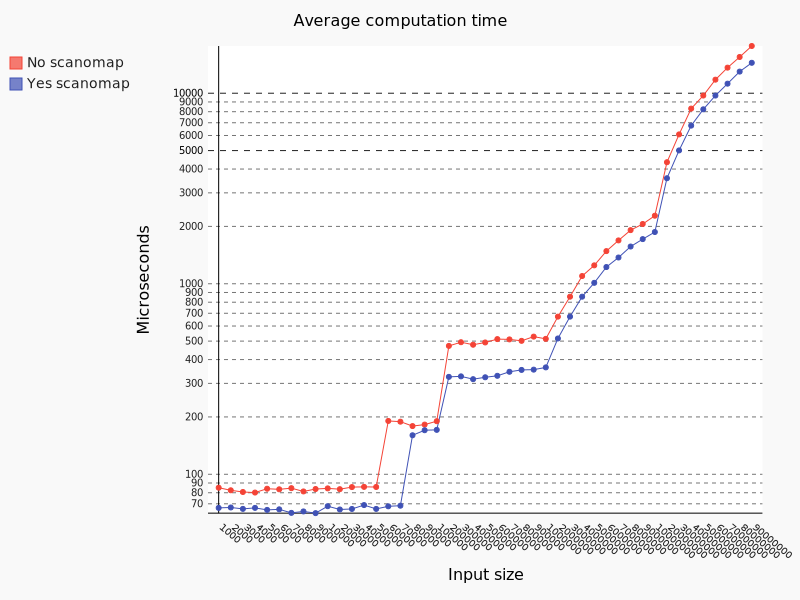
\includegraphics[width=0.9\textwidth]{images/chart.png}
  \caption{Computation time for Map-Scan Fusion test}
  \label{fig:map-scan fusion test}
\end{figure}

Figure \ref{fig:map-scan fusion speedup} shows the speedup with scanomap, and the immediate result shows that with the scanomap implementation the computation is approximately 1.35 times faster. For data larger than 5,000,000 the speedup seems to stay about 1.2 times faster. We have not identified the cause of the two high spikes at 60,000 and 70,000 data sizes, as we do not believe it is relevant to our work.

\begin{figure}[h!]
  \centering
    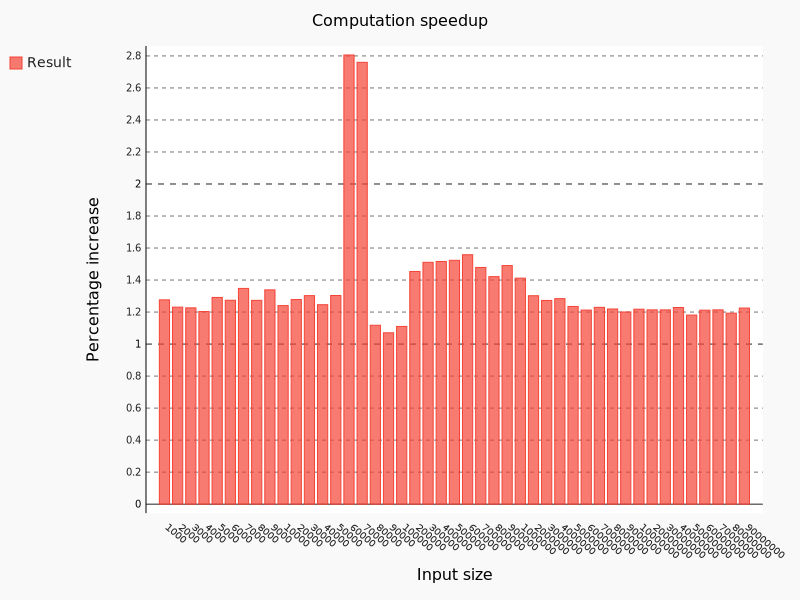
\includegraphics[width=0.9\textwidth]{images/comparing.png}
  \caption{Speedup chart}
  \label{fig:map-scan fusion speedup}
\end{figure}

\paragraph*{CPU:} When running the same test on the CPU, we see that the \texttt{scanomap} is no longer consistantly faster. Below input size of 20,000, the computation time is faster without \texttt{scanomap} as seen in Figure \ref{fig:CPU-map-scan fusion speedup}. With input sizes higher than 20,000, and especially above 100,000, scanomap gives a significant speedup.

\begin{figure}[h!]
  \centering
    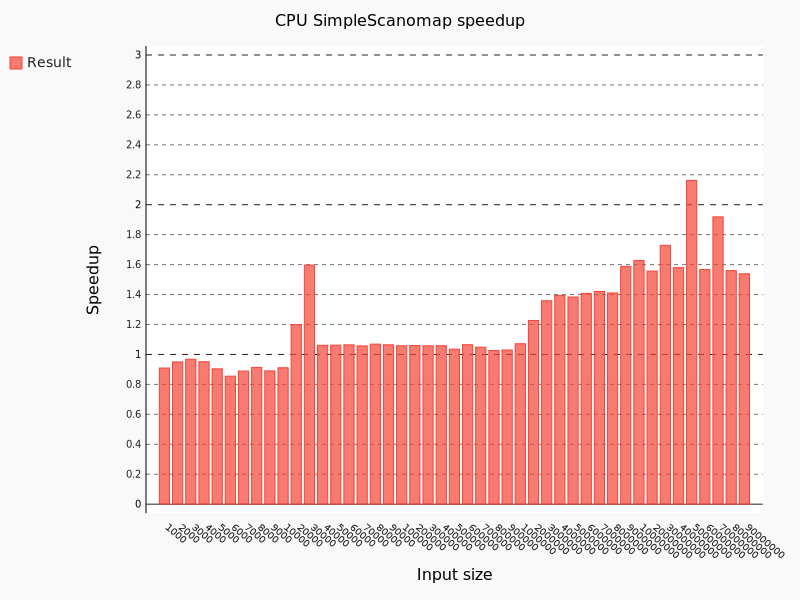
\includegraphics[width=0.9\textwidth]{images/futhark-c-comparing.png}
  \caption{Speedup chart}
  \label{fig:CPU-map-scan fusion speedup}
\end{figure}

\paragraph*{Radix sort:}

To benchmark the scanomap implementation with a more complicated program that does more work, we have benchmarked the radix sort Futhark program (Appendix A). The results displayed in Figure \ref{fig:scanomap-radix} show considerable speedup with an average of 1.32 times faster than without scanomap.

\begin{figure}[hb]
  \centering
    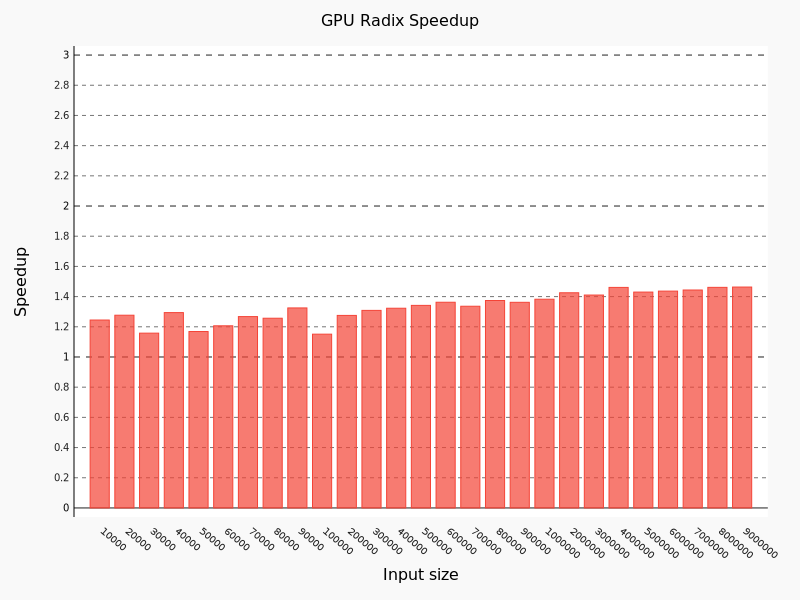
\includegraphics[width=0.9\textwidth]{images/radix-comparing.png}
  \caption{Radix-Speedup chart}
  \label{fig:scanomap-radix}
\end{figure}

\paragraph*{Scanomap-Scanomap fusion:}
To test the effect of implementing the horizontal fusion of scanomap-scanomap, we have made a Futhark program and tested it in three ways:

\begin{itemize}
\item Without any fusion.
\item With scanomap fusion.
\item With scanomap fusion and scanomap-scanomap fusion.
\end{itemize}

\begin{lstlisting}[caption=Scanomap-scanomap benchmark program] 
fun [int, n] main([int, n] inp) =
    let a  = map(+10, inp) in
    let b1 = scan(+, 0, a) in
    let a2 = map(+1, a) in
    let b2 = scan(+, 0, a2) in
    map(fn int (int x,int y) => x + y, zip(b1,b2))

\end{lstlisting}

\begin{figure}[hb]
  \centering
    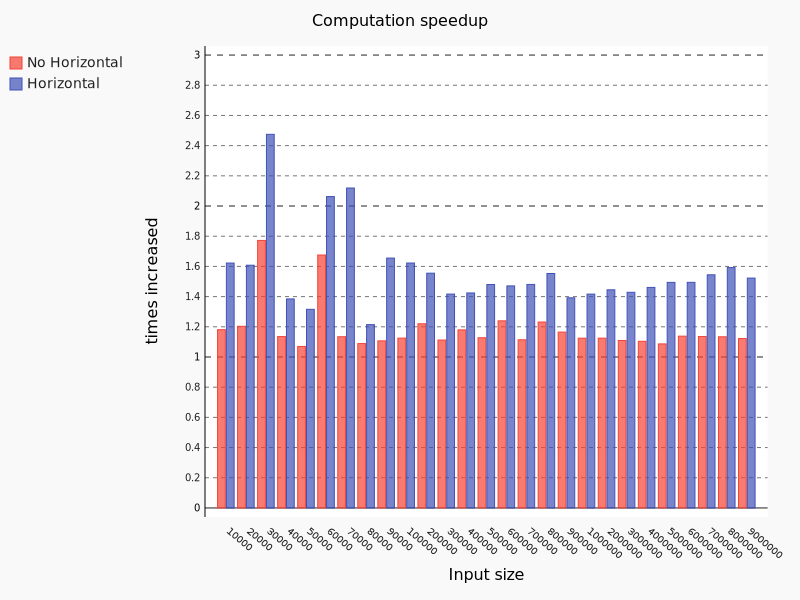
\includegraphics[width=0.9\textwidth]{images/horri-comparing.png}
  \caption{Speedup chart for scanomap-scanomap fusion benchmark}
  \label{fig:scanomap-scanomap}
\end{figure}

The results in Figure \ref{fig:scanomap-scanomap} show a speedup of average 1.19 times faster by using scanomap fusion, illustrated by the red bars. However, by adding the \texttt{scanomap}-\texttt{scanomap} fusion illustrated by the blue bars, the results are an average of 1.56 times faster computation.

\clearpage
\newpage
\section{Future Work}
There is a potential to expand the \texttt{scanomap} construct to accommodate more fusion. Currently the \texttt{scanomap} construct supports fusion as a consumer with a producer \texttt{map} as well
 as horizontal fusion with another \texttt{scanomap}. However, as we can see in Listings \ref{lst:maposcanomap1} and \ref{lst:mos1}, it makes sense
 -- at least sequentially -- to think of fusing \texttt{scanomap} as producer into
 a consumer \texttt{map}. Futhermore, it should also be possible to exploit this fusion in parallel computation.

\begin{lstlisting}[caption=$\mathtt{scanomap} \: g \: g_f \: ne \: a$ and $\mathtt{map} \: h \: b$ as sequential loops., label={lst:maposcanomap1}]
  a[n];
  ...
  b[n];
  acc = e;
  for (int i = 0; i < n; i++) {
    acc = g(acc, f(a[i]));
    b[i] = acc;
  }
  c[n];
  for (int i = 0; i < n; i++) {
    c[i] = f(b[i]);
  }
\end{lstlisting}

\begin{lstlisting}[caption=Listing \ref{lst:maposcanomap1} fused., label={lst:mos1}]
  a[n];
  ...
  c[n];
  acc = e;
  for (int i = 0; i < n; i++) {
    acc = g(acc, f(a[i]));
    c[i] = h(acc);
  }
\end{lstlisting}
Supporting \texttt{scanomap}-\texttt{map} fusion would require an expansion of the \texttt{scanomap} construct, adding a third function. This would alter \texttt{scanomap}'s type signature to,
$$\mathtt{scanomap} \: \odot \: \odot_f \: g \: e \: a \: : \:(\alpha \to \alpha \to \alpha) \to (\alpha \to \beta \to \alpha)
 \to (\alpha \to \gamma) \to \alpha \to [\beta] \to [\gamma]\mathnormal{.}$$
and semantically change such that the function $g$ is applied as the final step,
$$\mathtt{scanomap} \: \odot \: \odot_f \: e \: a \: =
 [g(e \odot_f a_0), g((e \odot_f a_0) \odot_f a_1), ..., g(((e \odot_f a_0) \odot_f ...) \odot_f a_{n-1})]\mathnormal{.}$$
Any old \texttt{scanomap} can then be represented in the new construct by simply setting $g$ to be the identity function $g(x) = x$, and as such it would not require much work to uphold the
 existing \texttt{map}-\texttt{scan} implementation. Horizontal fusion between two \texttt{scanomap}s would also work with slight modifications, for example composing their third functions.

With the altered \texttt{scanomap}, performing \texttt{scanomap}-\texttt{map} fusion would be as simple as performing function composition between the new \texttt{scanomap} function and 
the \texttt{map} function. Implementation would be similar to what can be seen in Section \ref{sec:imp}.
 \begin{align*}
   \lett b &= \mathtt{scanomap} \: \odot \: \odot_f \: g \: ne \: a \inn \\
   \lett c &= \mathtt{map} \: h \: b \inn \\
   &\vdots \\
   \lett c &= \mathtt{scanomap} \: \odot \: \odot_f \: (h \circ g) \: ne \: a \inn
 \end{align*}
The results of this project imply that we could experience similar speedups when performing \texttt{scanomap}-\texttt{map} fusion. Therefore, we think that exploring this possibility
 would be a worthwhile pursuit.
\clearpage
\section{Conclusion}
Exploiting invariants inherent in \texttt{map} and \texttt{scan} as well creating the \texttt{scanomap} construct has allowed us
 to fairly simply define an algorithm for performing \texttt{map}-\texttt{scan} fusion. This algorithm allows for any two compatible
 producer-consumer, \texttt{map}s and \texttt{scan}s to be fused into a single \texttt{scanomap}. Moreover, we have shown
how a \texttt{scanomap}  can
 be further fused as a consumer with a producer \texttt{map}, as well as horisontally with another \texttt{scanomap}.

We have benchmarked Futhark programs with and without our additions to the Futhark compiler, and have documented a GPU speedup in the range 1.2-1.5 times faster for fused programs compared to their pre-\texttt{scanomap} implementation counterparts.

 Additionally, our implementation of \texttt{scanomap} has also opened the door for more fusion optimisations. We sketched how
 \texttt{scanomap}-\texttt{map} fusion, is a candidate for future work, with the chance of improving execution time even further.
\newpage

\bibliographystyle{unsrt}
\bibliography{lit}

\newpage
\section{Appendix}
\subsection{A - Radix sort}
\begin{lstlisting}[caption=Test program] 
fun [u32, n] main([u32, n] xs) =
  radix_sort(xs)

fun [u32, n] radix_sort([u32, n] xs) =
  loop (xs) = for i < 32 do
    radix_sort_step(xs, i)
  in xs

fun [u32, n] radix_sort_step([u32, n] xs, i32 digit_n) =
  let bits = map(fn i32 (u32 x) => i32((x >> u32(digit_n)) & 1u32), xs)
  let bits_inv = map(fn i32 (i32 b) => 1 - b, bits)
  let ps0 = scan(+, 0, bits_inv)
  let ps0_clean = map(*, zip(bits_inv, ps0))
  let ps1 = scan(+, 0, bits)
  let ps0_offset = reduce(+, 0, bits_inv)
  let ps1_clean = map(+ ps0_offset, ps1)
  let ps1_clean' = map(*, zip(bits, ps1_clean))
  let ps = map(+, zip(ps0_clean, ps1_clean'))
  let ps_actual = map(fn i32 (i32 p) => p - 1, ps)
  in write(ps_actual, xs, copy(xs))

\end{lstlisting}

\newpage
\subsection{B - Implementation code}
Examples of the code for implementing scanomap fusion. This is not the complete code.

\subsubsection{Implementaion of scanomap SOAC}

\begin{lstlisting}[language=Haskell,caption=Implementing scanomap as SOAC] 
-- | A definite representation of a SOAC expression.
data SOAC lore = Map Certificates SubExp (Lambda lore) [Input]
               | Reduce Certificates SubExp Commutativity (Lambda lore) [(SubExp,Input)]
               | Scan Certificates SubExp (Lambda lore) [(SubExp,Input)]
               | Redomap Certificates SubExp Commutativity (Lambda lore) (Lambda lore) [SubExp] [Input]
               | Scanomap Certificates SubExp (Lambda lore) (Lambda lore) [SubExp] [Input]
               | Stream Certificates SubExp (StreamForm lore) (Lambda lore) [Input]
            deriving (Show)
            
-- | Returns the inputs used in a SOAC.
inputs :: SOAC lore -> [Input]
inputs (Scanomap _ _ _ _ _  arrs) = arrs

-- | Set the inputs to a SOAC.
setInputs :: [Input] -> SOAC lore -> SOAC lore
setInputs arrs (Scanomap cs w lam1 lam ne _) =
  Scanomap cs w lam1 lam ne arrs
  
-- | The lambda used in a given SOAC.
lambda :: SOAC lore -> Lambda lore
lambda (Scanomap _ _ _ lam2 _ _) = lam2

-- | Set the lambda used in the SOAC.
setLambda :: Lambda lore -> SOAC lore -> SOAC lore
setLambda lam (Scanomap cs w lam1 _ ne arrs) =
  Scanomap cs w lam1 lam ne arrs


-- | Returns the certificates used in a SOAC.
certificates :: SOAC lore -> Certificates
certificates (Scanomap cs _ _ _ _ _)  = cs

-- | The return type of a SOAC.
typeOf :: SOAC lore -> [Type]
typeOf (Scanomap _ w outlam inlam nes _) =
  let accrtps = mapType w outlam
      arrrtps = drop (length nes) $ mapType w inlam
  in  accrtps ++ arrrtps

width :: SOAC lore -> SubExp
width (Scanomap _ w _ _ _ _) = w

-- | Convert a SOAC to the corresponding expression.
toExp :: (MonadBinder m, Op (Lore m) ~ Futhark.SOAC (Lore m)) =>
         SOAC (Lore m) -> m (Exp (Lore m))
toExp (Scanomap cs w l1 l2 es as) =
  Op <$> (Futhark.Scanomap cs w l1 l2 es <$> inputsToSubExps as)

-- | Either convert an expression to the normalised SOAC
-- representation, or a reason why the expression does not have the
-- valid form.
fromExp :: (Bindable lore, Op lore ~ Futhark.SOAC lore, HasScope t f) =>
           Exp lore -> f (Either NotSOAC (SOAC lore))

fromExp (Op (Futhark.Map cs w l as)) =
  Right . Map cs w l <$> traverse varInput as
fromExp (Op (Futhark.Reduce cs w comm l args)) = do
  let (es,as) = unzip args
  Right . Reduce cs w comm l . zip es <$> traverse varInput as
fromExp (Op (Futhark.Scan cs w l args)) = do
  let (es,as) = unzip args
  Right . Scan cs w l . zip es <$> traverse varInput as
fromExp (Op (Futhark.Redomap cs w comm l1 l2 es as)) =
  Right . Redomap cs w comm l1 l2 es <$> traverse varInput as
fromExp (Op (Futhark.Scanomap cs w l1 l2 es as)) =
  Right . Scanomap cs w l1 l2 es <$> traverse varInput as
fromExp (Op (Futhark.Stream cs w form extlam as)) = do
  let mrtps = map hasStaticShape $ extLambdaReturnType extlam
      rtps  = catMaybes mrtps
  if length mrtps == length rtps
  then Right <$> do let lam = Lambda (extLambdaParams extlam)
                                     (extLambdaBody extlam)
                                     rtps
                    Stream cs w form lam <$> traverse varInput as
  else pure $ Left NotSOAC
fromExp _ = pure $ Left NotSOAC
\end{lstlisting}

\newpage
\subsubsection{Implementing scanomap in loop kernel}
\begin{lstlisting}[language=Haskell,caption=Scanomap implementation in loop kernel] 
removeUnusedParamsFromKer :: FusedKer -> FusedKer
removeUnusedParamsFromKer ker =
  case soac of
    SOAC.Map {}     -> ker { fsoac = soac' }
    SOAC.Redomap {} -> ker { fsoac = soac' }
    SOAC.Scanomap {} -> ker { fsoac = soac' }
    _               -> ker
  where soac = fsoac ker
        l = SOAC.lambda soac
        inps = SOAC.inputs soac
        (l', inps') = removeUnusedParams l inps
        soac' = l' `SOAC.setLambda`
                (inps' `SOAC.setInputs` soac)
                
   ----------------------------
    -- Scanomap Fusions:      --
    ----------------------------

    (SOAC.Scanomap _ _ lam2r _ nes2 _, SOAC.Scanomap _ _  lam1r _ nes1 _)
      | horizFuse -> do
          let (res_lam', new_inp) = fuseRedomap unfus_set outVars nes1 lam1 inp1_arr outPairs lam2 inp2_arr
              unfus_accs  = take (length nes1) outVars
              unfus_arrs  = returned_outvars \\ unfus_accs
              lamr        = mergeReduceOps lam1r lam2r
          success (unfus_accs ++ outNames ker ++ unfus_arrs) $
              SOAC.Scanomap (cs1++cs2) w  lamr res_lam' (nes1++nes2) new_inp

    -- Map -> Scanomap Fusion
    (SOAC.Scanomap _ _ lam21 _ nes _, SOAC.Map {})
      | mapFusionOK outVars ker || horizFuse -> do
      -- Create new inner reduction function
      let (res_lam, new_inp) = fuseMaps unfus_set lam1 inp1_arr outPairs lam2 inp2_arr
          -- Get the lists from soac1 that still need to be returned
          (_,extra_rtps) = unzip $ filter (\(nm,_)->nm `HS.member` unfus_set) $
                           zip outVars $ map (stripArray 1) $ SOAC.typeOf soac1
          res_lam' = res_lam { lambdaReturnType = lambdaReturnType res_lam ++ extra_rtps }
      success (outNames ker ++ returned_outvars) $
              SOAC.Scanomap (cs1++cs2) w lam21 res_lam' nes new_inp
  
  
              
scanToScanomap :: Maybe [VName] -> SOAC -> SOAC.ArrayTransforms
               -> TryFusion (SOAC, SOAC.ArrayTransforms)
scanToScanomap _ (SOAC.Scan cs w scan_fun scan_input) ots = do
       let (nes, array_inputs) =  unzip scan_input
       return (SOAC.Scanomap cs w scan_fun scan_fun nes array_inputs, ots)
scanToScanomap _ _ _ =
  fail "Only turn scan into scanomaps"
\end{lstlisting}

\subsubsection{Implementing first order transform scanomap}
\begin{lstlisting}[language=Haskell,caption=Scanomap first order transform] 
transformSOAC pat (Scanomap cs width _ fun accexps arrexps) = do
  i <- newVName "i"
  -- Name accumulators, do something with the corresponding expressions
  (acc, initacc, _) <- newFold "scanomap" (zip accexps accts) arrexps
  -- Create output arrays.
  initarr <- resultArray scan_res_ts
  -- Name Outputarrays?
  arr <- mapM (newIdent "scan_arr" ) scan_res_ts
  -- Create arrays for our map results.
  initmaparrs <- resultArray map_res_ts
  mapoutarrs <- mapM (newIdent "scanomap_map_outarr") map_res_ts
  -- Get the names
  let arr_names = map identName arr
      map_names = map identName mapoutarrs
      merge = loopMerge (acc++arr++mapoutarrs) (initacc++map Var initarr ++ map Var initmaparrs)
  loopbody <- insertBindingsM $ localScope (scopeOfFParams $ map fst merge) $ do
    -- Bind function parameters to arguments.
    x <- bindLambda fun (map (PrimOp . SubExp . Var . identName) acc ++
                              index cs arrexps (Var i))
    -- Set function destinations
    dests <- letwith cs arr_names (pexp (Var i)) $ map (PrimOp . SubExp) (take (length accexps) x)
    mapdests <- letwith cs map_names (pexp (Var i)) $ map (PrimOp . SubExp) (drop (length accexps) x)
    irows <- letSubExps "row" $ index cs dests $ Var i
    rowcopies <- mapM copyIfArray irows
    return $ resultBody $ rowcopies ++ map Var dests ++ map Var mapdests
  pat' <- discardPattern (map identType acc) pat
  letBind_ pat' $ DoLoop [] merge (ForLoop i width) loopbody
  where accts = map paramType $ take (length accexps) $  lambdaParams fun
        scan_res_ts = [ arrayOf t (Shape [width]) NoUniqueness
                     | t <- (take (length accexps) (lambdaReturnType fun))]
        map_res_ts = [ arrayOf t (Shape [width]) NoUniqueness
                     | t <- (drop (length accexps) (lambdaReturnType fun))]
\end{lstlisting}
\end{document}